\begin{itemize}

\item Self energy inclusion suppresses the charge channel in favor of FM fluctuations

\item Self energy lowers the critical scale

\end{itemize}

\begin{figure}
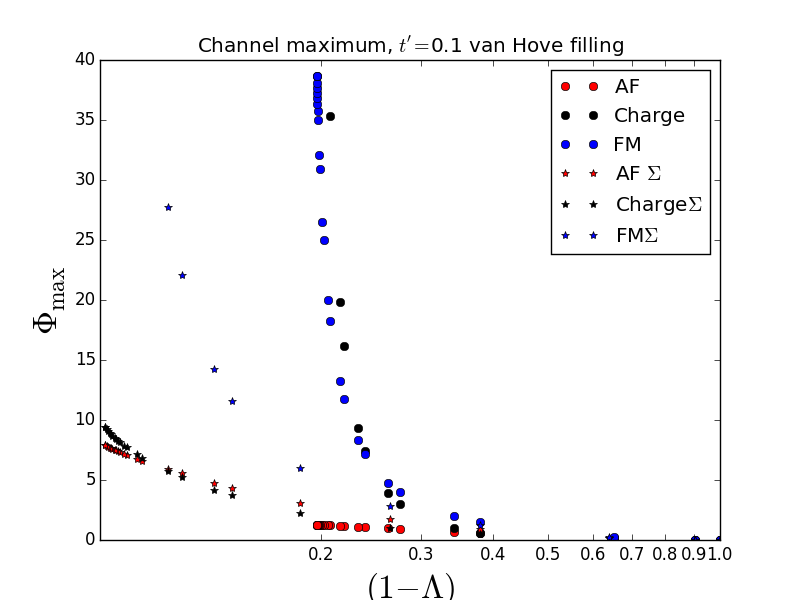
\includegraphics[scale=0.5]{images/sevsnose.png}
\caption{Max values of the channels as functions of cutoff scale, with and without self energy. }
 \end{figure}
 
 \begin{figure}
 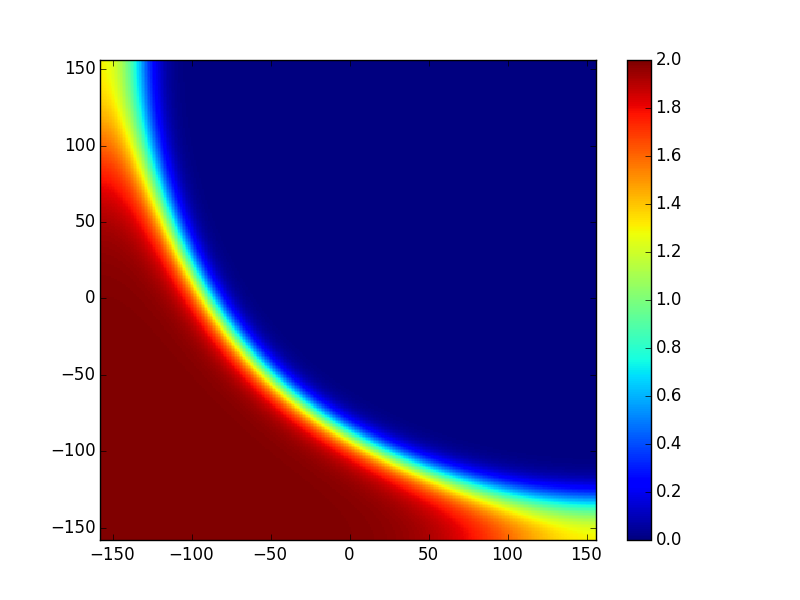
\includegraphics[scale=0.5]{images/Fermi_occupation_nose.png}
 \caption{Non interacting Fermi occupation in the BZ. }
 \end{figure}
 
  \begin{figure}
 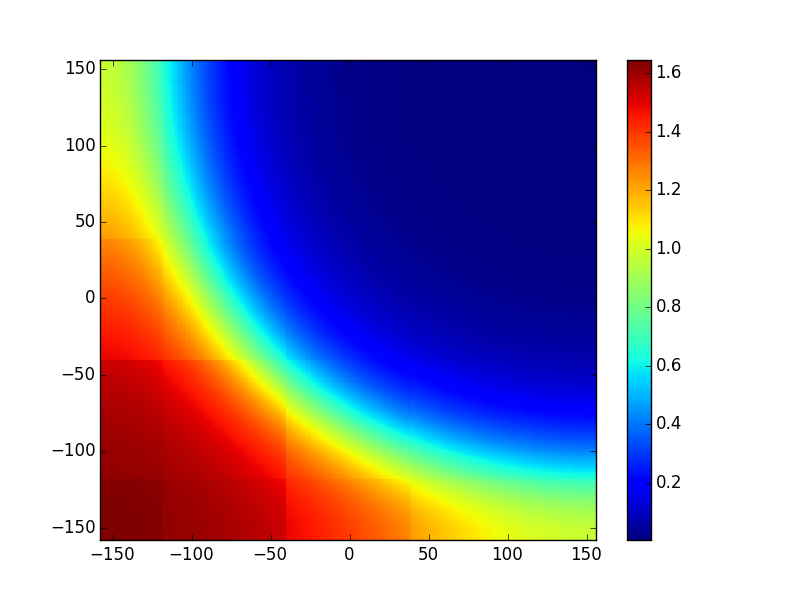
\includegraphics[scale=0.5]{images/Fermi_occupation_se.png}
 \caption{Interacting Fermi occupation in the BZ. }
 \end{figure}